% Visual redesign only. Original measured values, baseline, margins and objective unchanged.
% Compile with an existing XeLaTeX installation from this directory:
% xelatex -interaction=nonstopmode -halt-on-error technical_note_v2.tex
\RequirePackage{fix-cm}
\documentclass[11pt,a4paper]{article}
\usepackage[margin=17mm]{geometry}
\usepackage{fontspec}
\setmainfont{Arial}
\setsansfont{Arial}
\setmonofont{Arial}
\usepackage{graphicx}
\usepackage{xcolor}
\usepackage{array}
\usepackage{enumitem}
\usepackage{hyperref}
\definecolor{ink}{HTML}{203642}
\definecolor{teal}{HTML}{167C80}
\definecolor{muted}{HTML}{536B78}
\definecolor{lightgray}{HTML}{DDE5E8}
\hypersetup{colorlinks=true,urlcolor=muted,linkcolor=muted,pdfauthor={Zhijing Wu},pdftitle={When Can Communication Cost Change a Local Protocol Assignment? A Reproducible Diagnostic on ProtocolBench}}
\pagestyle{empty}
\setlength{\parindent}{0pt}
\setlength{\parskip}{2pt}
\setlength{\columnsep}{8mm}
\newlength{\gridcol}
\setlength{\gridcol}{\dimexpr\textwidth/2-\columnsep/2\relax}
\newcommand{\bodyfont}{\fontsize{11}{15}\selectfont}
\newcommand{\auxfont}{\fontsize{9.5}{12.5}\selectfont}
\newcommand{\sectionlabel}[1]{\par{\fontsize{13}{16}\selectfont\bfseries #1}\par\vspace{6pt}}
\newcommand{\indextext}[1]{\raisebox{-0.35ex}{\auxfont #1}}
% The equation uses Arial glyphs, including its Unicode sum/Greek symbols.
% This avoids adding a second visual font family for the mathematical notation.
\newcommand{\sumop}[1]{\raisebox{-1.0ex}{\begin{tabular}[b]{@{}c@{}}{\fontsize{17}{18}\selectfont ∑}\\[-2pt]{\auxfont #1}\end{tabular}}}
\newcommand{\finding}[3]{\noindent\hangindent=10mm\hangafter=1\makebox[10mm][l]{\color{teal}#1}\textbf{#2}\enspace #3\par\vspace{10pt}}
\setlist[itemize]{leftmargin=12pt,itemsep=3pt,topsep=5pt,parsep=0pt,label=\textbullet}
\begin{document}
\color{ink}\bodyfont

% PAGE 1: one dominant mechanism schematic.
{\fontsize{22}{25}\selectfont\bfseries
When Can Communication Cost Change\\
a Local Protocol Assignment?\par}
\vspace{3pt}
{\fontsize{13}{16}\selectfont\color{muted}
A Reproducible Diagnostic on ProtocolBench\par}
\vspace{4pt}
{\auxfont
Zhijing Wu\enspace·\enspace Sichuan University\enspace·\enspace CS undergraduate\enspace·\enspace
\href{mailto:zhijing.wu.cs@gmail.com}{zhijing.wu.cs@gmail.com}\enspace·\enspace
\href{https://zhijingwu.github.io}{zhijingwu.github.io}\par}
\vspace{10pt}

% V01--V04: the same audited call, runtime dependency and modeled question as v1.
{\raggedright At commit \href{https://github.com/ulab-uiuc/AgentProtocols/tree/6349eb97f0ca83db9cbfd44dea0bbdbb3ea9d37f}{6349eb97},
I noticed that the audited released GAIA assignment call receives task/agent inputs
without explicit graph or edge-demand input; its caller uses the original heuristic
fallback. Runtime communication follows destination-specific protocol paths and
records request metrics. I asked whether measured local communication cost and
controlled demand can change the minimizer of a declared assignment objective,
with the saved baseline and synthetic margins held fixed.\par}

\vspace{9pt}
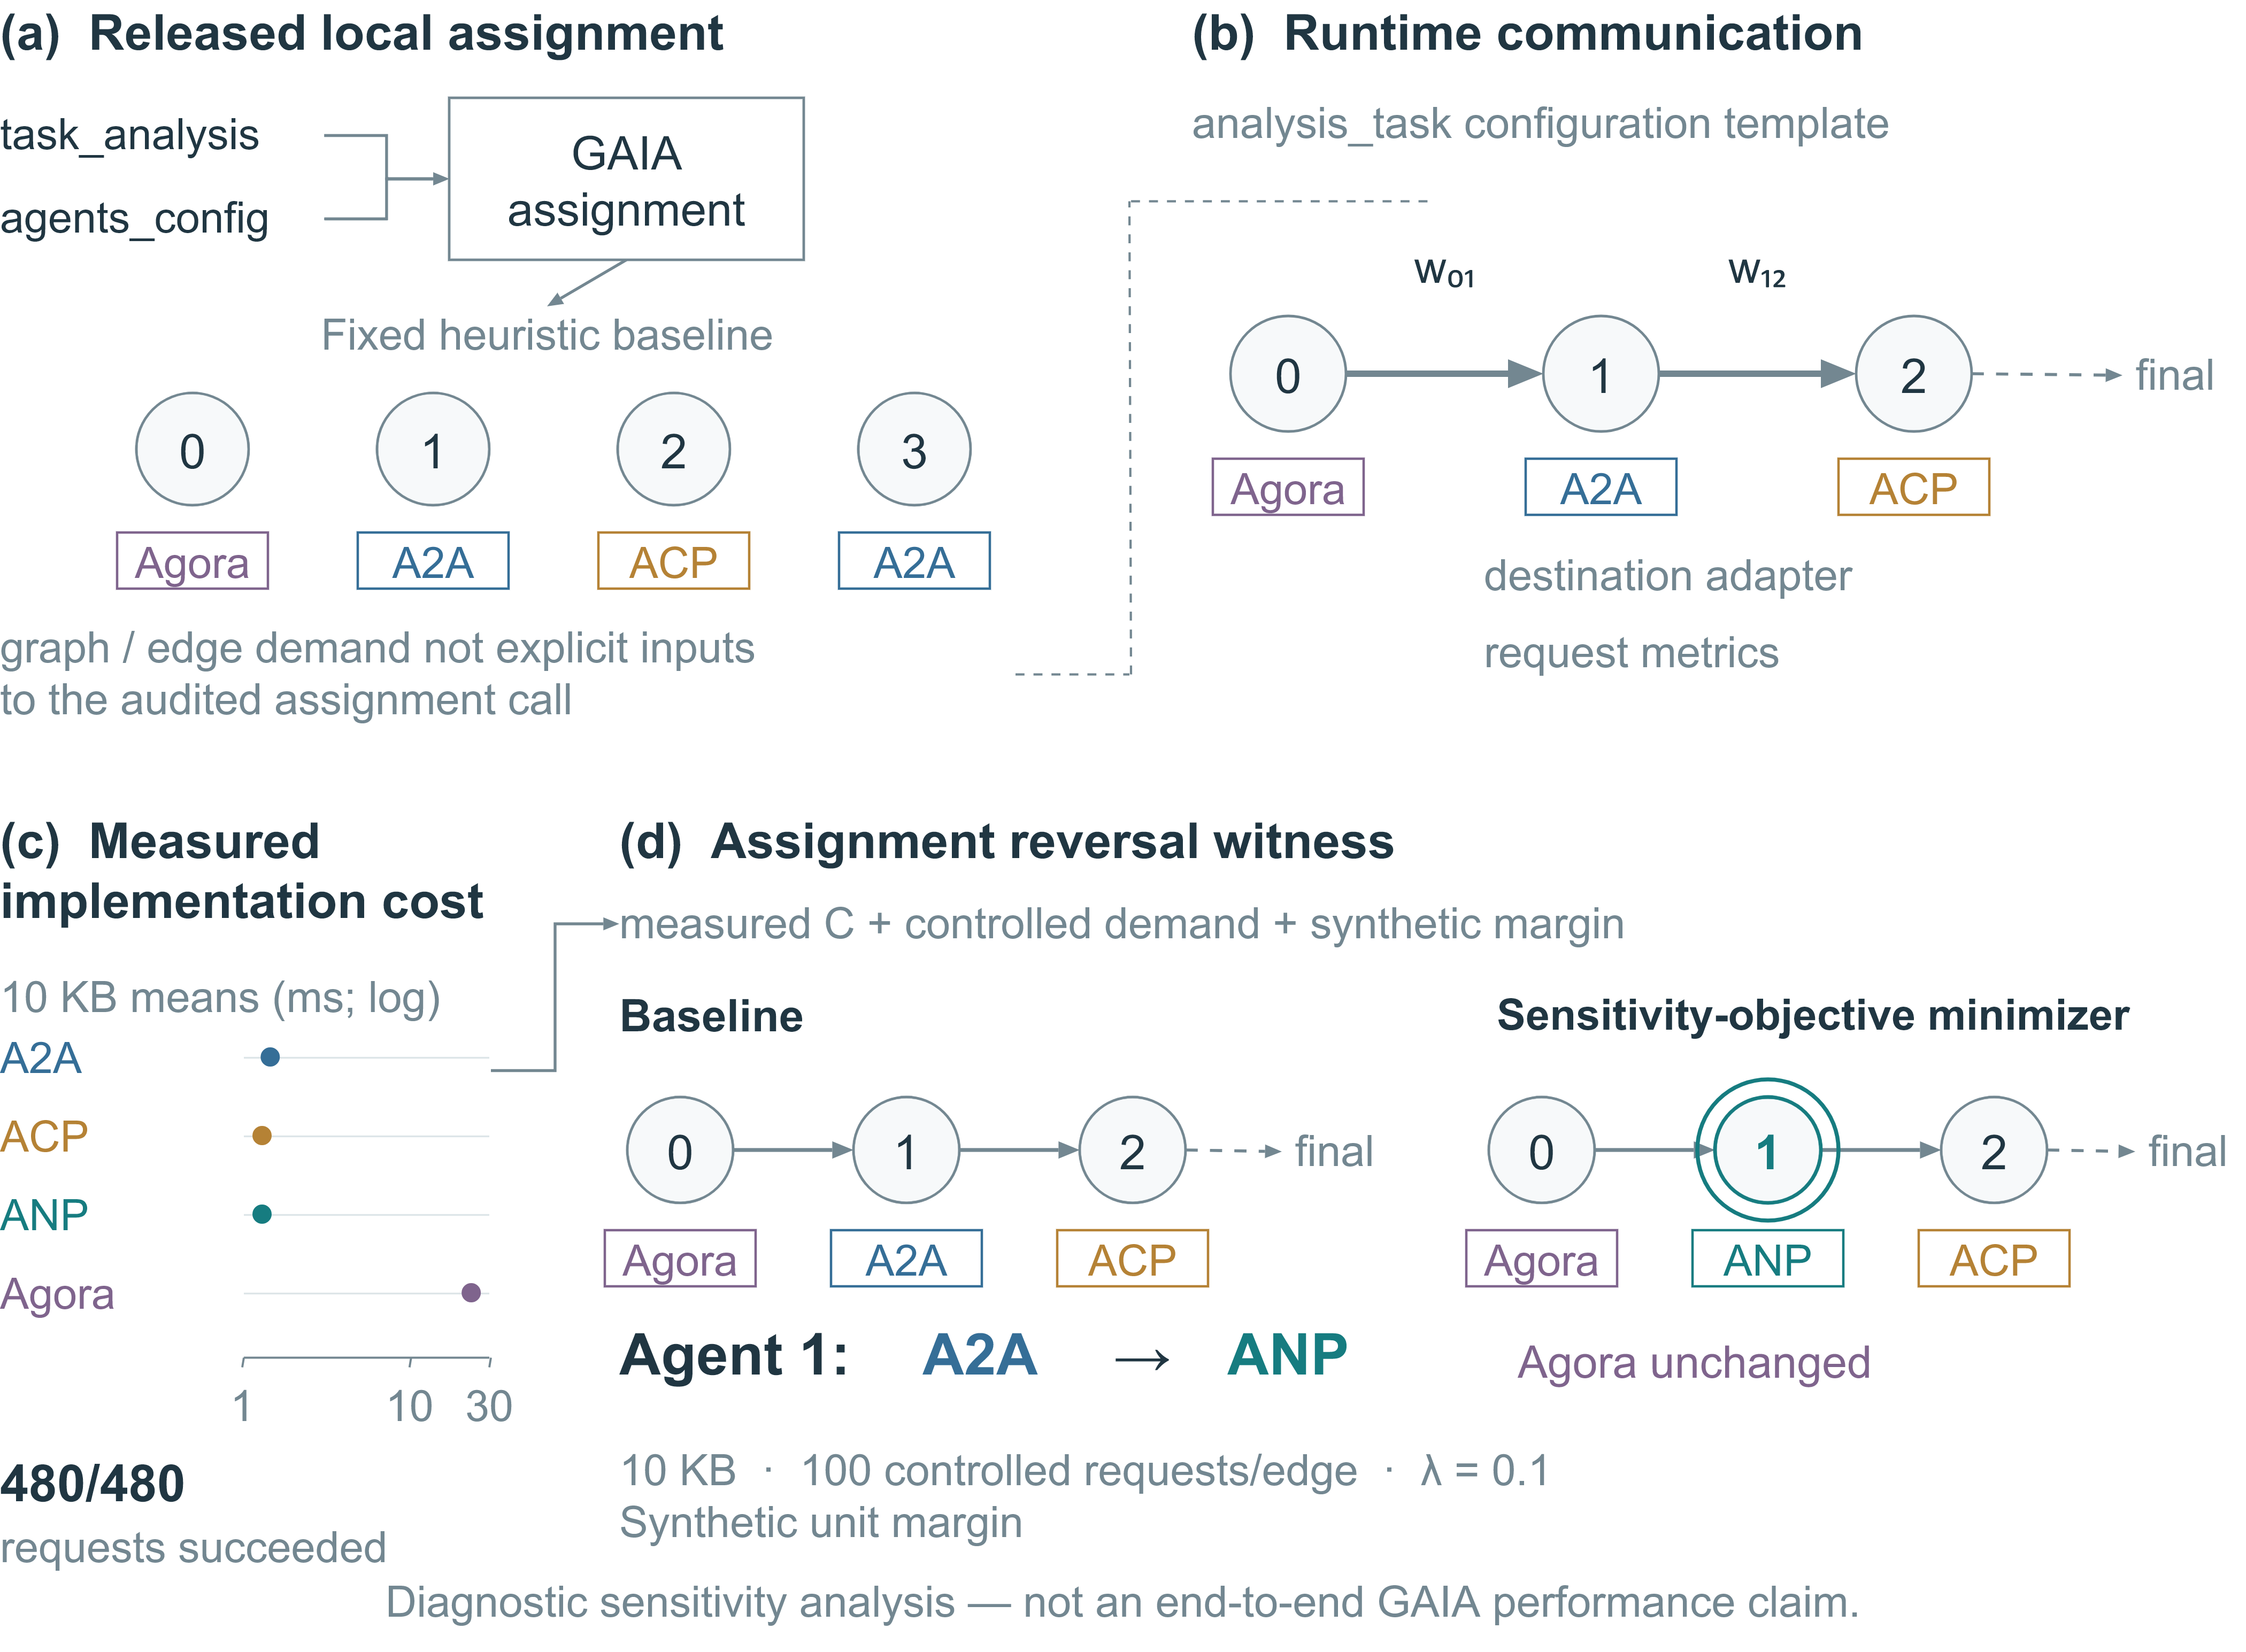
\includegraphics[width=\textwidth]{figures/protocol_assignment_mechanism.png}\par
\vspace{3pt}
{\auxfont\color{muted}\raggedright
% V05: disclosed official template, not runtime trace.
The official analysis\_task configuration template is instantiated under disclosed
conventions; final is terminal output, not another agent. Agent 3 remains A2A
outside this template's edges.\par}
\vspace{9pt}

\sectionlabel{What I found}
% V06--V08: all saved results; no new scientific runs.
\finding{01}{Real runtime paths.}{480/480 measured requests succeeded across all four protocols.}
\finding{02}{Controlled graph sensitivity.}{37/144 configurations strictly changed the declared minimizer.}
\finding{03}{Repository-defined workflow.}{An eligible A2A→ANP reversal persists without Agora, with forced changes separated.}

\newpage

% PAGE 2: a fixed two-column grid, followed by a full-width interpretation.
\sectionlabel{Evidence and interpretation}
\vspace{3pt}
\begin{minipage}[t]{\gridcol}\raggedright
\sectionlabel{Measured protocol latency}
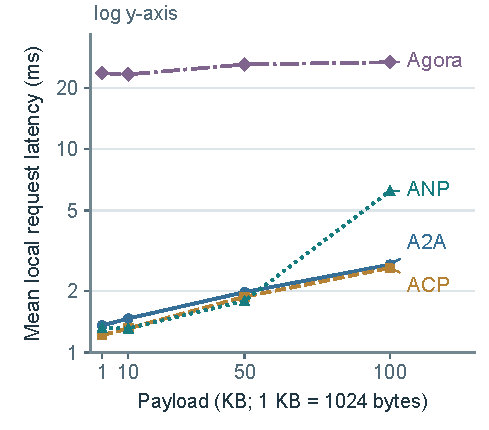
\includegraphics[width=\linewidth]{figures/protocol_latency_v2.pdf}\par
\vspace{4pt}
{\auxfont\color{muted}
% V09--V11: exact requested caption, one paragraph with a quiet qualifier.
Local no-op request latency through released repository client/server paths.
30 measured repetitions per protocol/size after 5 warmups; setup excluded.
HTTP/runtime-specific measurements; not intrinsic protocol rankings.\par}
\vspace{12pt}
% V12--V13: preserve the wall-clock boundary and uncertainty caveat.
Timing encloses BaseAgent.send, including encode/server/no-op/decode; no LLM.

ANP's 100 KB outlier is retained; close ACP/ANP mean differences do not establish
statistical superiority.
\end{minipage}\hspace{\columnsep}%
\begin{minipage}[t]{\gridcol}\raggedright
\sectionlabel{Declared sensitivity objective}
% V14: exact objective, set in the same Arial family as the document.
\vspace{1pt}
\begin{tabular}{@{}r@{\hspace{3pt}}l@{}}
J(\textbf{p}) =&\sumop{j} L\indextext{j}(p\indextext{j})\\[9pt]
&+ λ\,\sumop{(i,j) in E} w\indextext{ij}\,C(p\indextext{j},s\indextext{ij})
\end{tabular}\par
\vspace{7pt}
% V15--V18: inline legend, explicit conversion units.
\begin{tabular}{@{}p{8mm}@{}p{\dimexpr\linewidth-8mm\relax}@{}}
L\indextext{j}&synthetic local preference loss\\[4pt]
C&measured latency, ms/request\\[4pt]
w\indextext{ij}&controlled request demand\\[4pt]
λ&preference-loss units per accumulated ms
\end{tabular}\par
\vspace{12pt}

\sectionlabel{Representative witness}
% V19: original all-four analysis witness, unit margin unchanged.
\begin{tabular}{@{}p{20mm}@{}p{\dimexpr\linewidth-20mm\relax}@{}}
Workflow&analysis\_task\\[3pt]
Payload&10 KB\\[3pt]
Demand&100 requests/edge\\[3pt]
λ&0.1\\[3pt]
Margin&synthetic unit loss\\[3pt]
Change&\textbf{Agent 1: A2A→ANP}\\[3pt]
Agora&unchanged
\end{tabular}\par
\vspace{8pt}
% V20--V21: modeled result and forced-removal distinction.
The exhaustive oracle finds a changed minimizer of the declared objective;
this is not a GAIA task-quality claim.

Global Agora exclusion preserves this eligible reversal; forced agent-0 replacement
leaves no whole-assignment gain versus the original baseline in this analysis ablation.
\end{minipage}\par

\vspace{17pt}
\sectionlabel{What this establishes — and what it does not}
\begin{minipage}[t]{\gridcol}\raggedright
\textbf{Supported}
% V22--V25: scoped positive findings.
\begin{itemize}
\item Audited call: no explicit graph/edge-demand input.
\item Non-identical measured local runtime costs.
\item Declared objective admits reversals.
\item Eligible A2A→ANP reversal without Agora.
\end{itemize}
\end{minipage}\hspace{\columnsep}%
\begin{minipage}[t]{\gridcol}\raggedright
\textbf{Not established}
% V26--V31: identical scientific boundaries; the layout expands the three v1 bullets.
\begin{itemize}
\item GAIA task-quality improvement
\item Makespan improvement
\item Calibrated local utility or preference margins
\item Measured GAIA traffic traces
\item Universal protocol rankings
\item New routing-method superiority
\end{itemize}
\end{minipage}\par

\vspace{15pt}
\sectionlabel{Open question}
% V32: same signal gap; constraint-preserving study is conditional, not performed.
The public release does not expose graded agent×protocol preferences or validated
feasible-alternative masks for this GAIA path. If such signals are available,
would it be useful to study protocol assignment jointly with communication demand
under a constraint-preserving formulation?

I would be interested in exploring this direction further.

\vfill
{\auxfont\color{muted}\raggedright
% V33: citation previously verified against the official ICML listing.
[1] Hongyi Du et al. \textit{ProtocolBench}. ICML 2026.
\href{https://openreview.net/forum?id=GZRiXE2zBe}{OpenReview}.\\[3pt]
Code: \href{https://github.com/ulab-uiuc/AgentProtocols/tree/6349eb97f0ca83db9cbfd44dea0bbdbb3ea9d37f}{AgentProtocols @ 6349eb97}\enspace·\enspace
Claim audit: claim\_check\_v2.md\enspace·\enspace
Author: \href{https://github.com/ZhijingWu}{github.com/ZhijingWu}.
\par}
\end{document}
